% File: diary.tex
% Date: Mon Jun 17 19:58:29 2013 +0800
% Author: Yuxin Wu <ppwwyyxxc@gmail.com>
\section{过程记录}
\begin{enumerate}
    \item
首次出现正常的图片. 用了一个$ x-y$平面上的无限大平面及一个点光源。
此时仅仅参考\cite{phong}考虑了基本Phong模型中的漫反射与环境光,已经可以看到左下部分亮度较高,符合预期。

另外,远处的黑白纹理误差较大,不知是不可改进的浮点误差还是我的处理有误。
\begin{figure}[H]
  \centering
  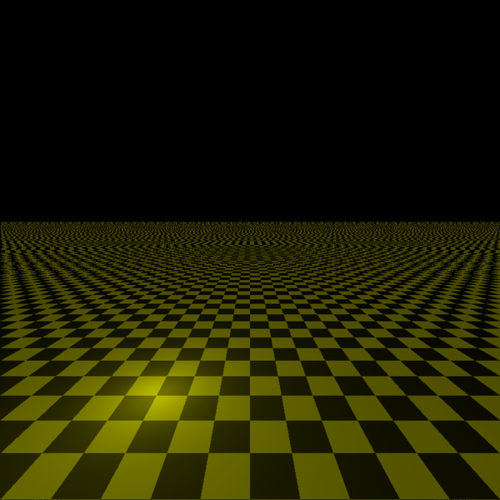
\includegraphics[scale=0.4]{res/first_pic.png}
  \caption{\label{fig:first}}
\end{figure}

\item
依照Beer-Lambert定律\cite{beer}对光线能量进行了按距离的减弱:
\[ E = E_0 e^{distance * density}\]
使得远处的纹理更自然.
\begin{figure}[H]
  \centering
  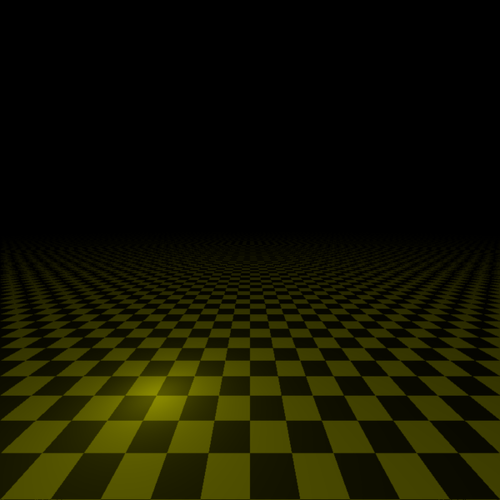
\includegraphics[scale=0.4]{res/plane_with_beer.png}
  \caption{\label{fig:beer}}
\end{figure}

\item

考虑了Phong模型中的高光,并对$ x-y$平面和$ y-z$平面加入了反射系数,有了互相反射的效果,并且
左下部分能够看到高光.打开\verb|-O3|编译开关时,在我的机器上渲染一张$600 \times 600$的图片需要0.39s.
\begin{figure}[H]
  \centering
  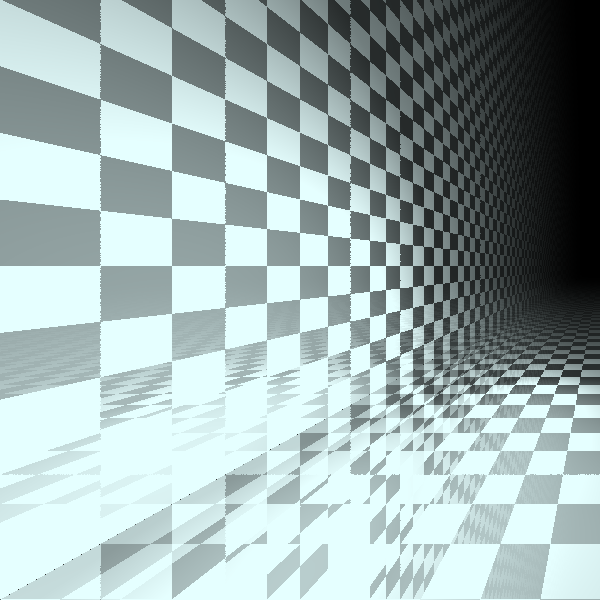
\includegraphics[scale=0.4]{res/specular.png}
  \caption{\label{fig:specular}}
\end{figure}

\item

  使用球模型,可以看到明显的高光效果。同时由于球面\verb|specular|参数高,使得球下部反射了平面。
\begin{figure}[H]
  \centering
  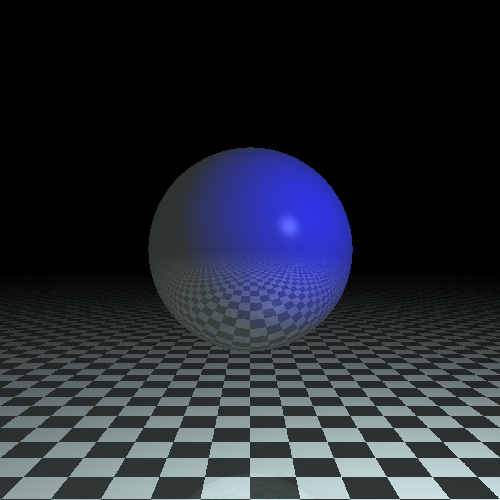
\includegraphics[scale=0.4]{res/ball.png}
  \caption{\label{fig:ball}}
\end{figure}

\item
  对于找到的交点,判断它与光源之间是否被挡住,若被挡住就不计算漫反射和高光. 这样实现了阴影效果.
\begin{figure}[H]
  \centering
  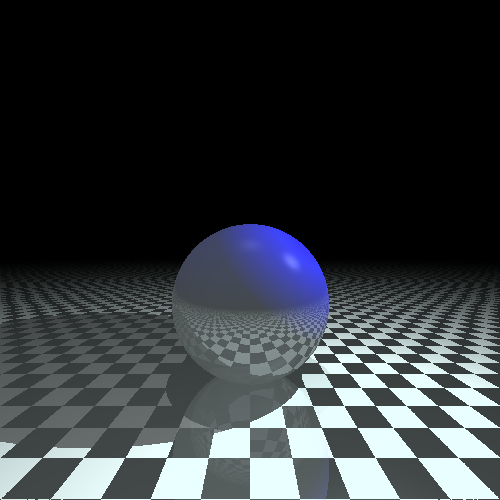
\includegraphics[scale=0.4]{res/shadow.png}
  \caption{\label{fig:shadow}}
\end{figure}

\item 对根据视点及对象生成视图(View)的方案进行修改,以支持视图的旋转,缩放.并利用opencv的key event实现了gui的旋转,缩放控制.
\begin{figure}[H]
  \centering
  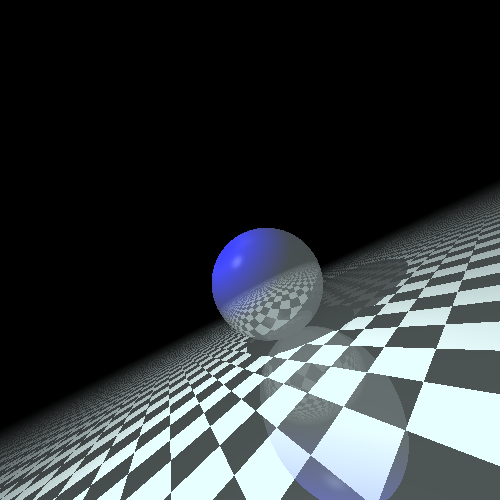
\includegraphics[scale=0.4]{res/rotate.png}
  \caption{\label{fig:rotate}}
\end{figure}

\item 加入了透射功能,依照预定义的介质密度及折射定律计算出射光方向.
\begin{figure}[H]
  \centering
  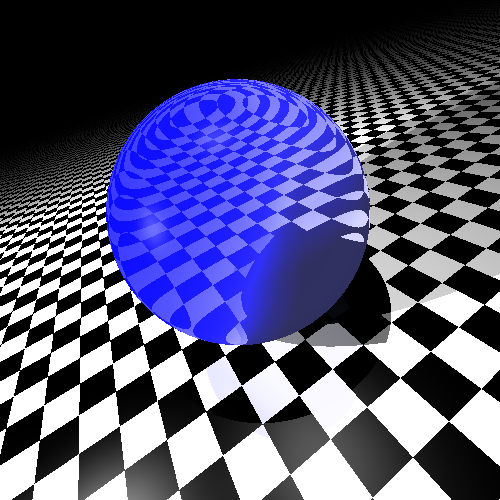
\includegraphics[scale=0.4]{res/transmission.png}
  \caption{\label{fig:transmission}}
\end{figure}

\item 实现了三角面片的渲染,在求交时计算齐次重心坐标,为网格中的法向插值做准备.
\begin{figure}[H]
  \centering
  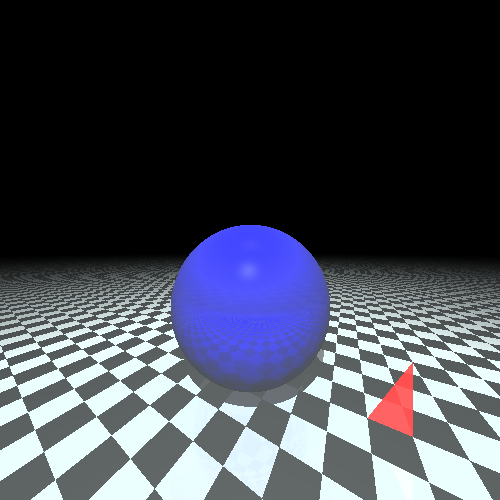
\includegraphics[scale=0.4]{res/face.png}
  \caption{\label{fig:face}}
\end{figure}

\item 实现了obj格式读取及基本的渲染,绘制出了一个红色小人.
\begin{figure}[H]
  \centering
  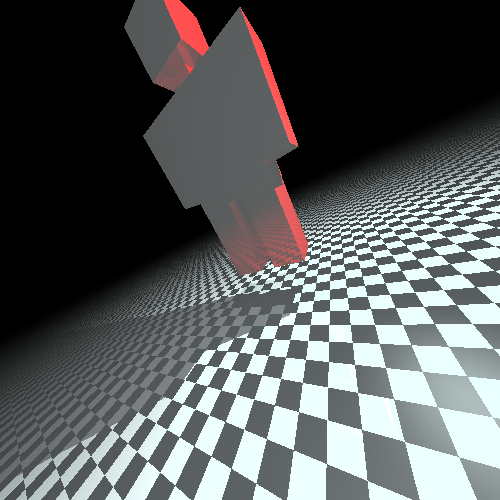
\includegraphics[scale=0.4]{res/human.png}
  \caption{\label{fig:human}}
\end{figure}

\item 实现了KDTree, 可以开始渲染更大的obj.
\begin{figure}[H]
  \centering
  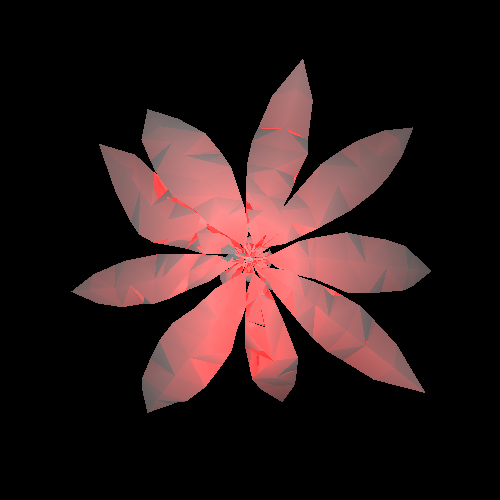
\includegraphics[scale=0.4]{res/flower.png}
  \caption{\label{fig:flower}}
\end{figure}

\item 按照\cite{kdtree}优化了KDTree的实现之后发现如下左图所示bug, 调试很久后发现两个原因.
  一是建树时选取候选切割平面未偏移\verb|EPS|, 二是包围盒求交存在小bug,少了一个绝对值运算.
  其中第二个bug还严重影响了速度.
\begin{figure}[H]
  \centering
\begin{minipage}[b]{0.46\linewidth}
  \centering
  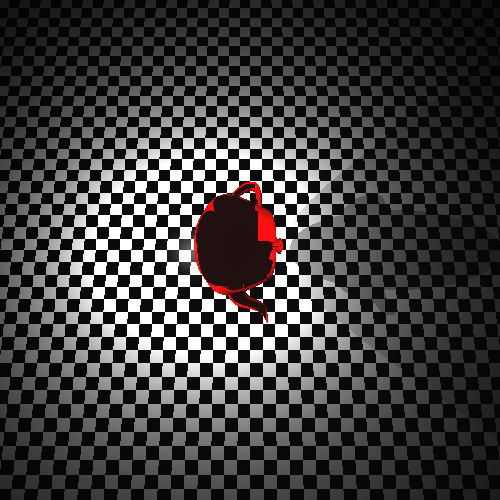
\includegraphics[width=\textwidth]{res/bug_teapot.png}
\end{minipage}
\begin{minipage}[b]{0.46\linewidth}
  \centering
  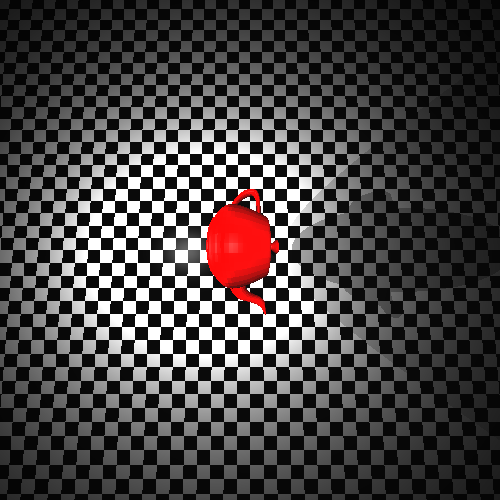
\includegraphics[width=\textwidth]{res/fixed_teapot.png}
\end{minipage}
  \caption{\label{fig:kdtree_bug}}
\end{figure}



\end{enumerate}
